\documentclass[12pt]{UoAthesis}
\thesistitle{Honours Dissertation}
\thesisauthor{Christopher James Thomson}
\thesispdfkeywords{}
\thesisyear{2012}

\thesisabstract{This is a short summary of my work...}
\acknowledgements{I would like to dedicate this work to..}

%%% The bibtex file where your references are stored
\bibliography{main}

\begin{document}

%%% = = = DISSERTATION OVERVIEW = = = %%%
% - Introduction - %
% - - Molecular dynamics, what is it, why is it important to Chemical
% - - engineering. Leading into potentials, need for faster methods,
% - - more accurate methods.
%
% Review of exisiting literature (Chapela, PRIME SPEADMD), what
% they've done, why its not as good as what you're going to do
%
% Outline of the thesis to come. 

% - Molecular Simulation
% -- Newtonian mechanics F=MA, is it valid?
% -- Forces from potentials (conservative forces)
% Types of forces (gravitional (which is neglected)), pairwise forces
% leading to intermolecular potentials.

% --- Give an example soft potential (LJ), Introduce a discrete --
% -potential, hard sphere is the prototypical discrete potential, --
% -but there are stepped potentials too (Chapela). Talk about the --
% -advantages/disadvantages etc.

%%%% Lead out of the chapter with this
% --- Introduce discrete potentials, say they need a special method of solution (EDMD).
% - Simulation Methods - %
% - - Force Driven Simulators
% - - - Introduction and general algorithm 
% - - - Integrators: Euler, Verlet, Velocity Verlet, Gear...lit review to find more recent ones
% - - - Optimization: neighbour lists, truncation of the potential 
% - - - Adv/Disadv? or just within other relevant topics
% - - Event Driven Simulators
% - - - Introduction and general algorithm
% - - - Collision rules
% Actually older than force based, although not as popular.
% - - - Optimization: neighbour lists, O(1) priority queue algorithms, time warp algorithms
% - - Measuring System Properties
% - - - Radial Distribution Function
% - - - Temperature
% - - - Pressure
% - - - Coefficient of Diffusion
% - Results - %
% - 'Checking the simulators' - %
%   Direct comparision with Chapela
% - Discussion - %
% - Conclusions - %
% - Recommendations for future work - %
% - Appendices - %
% - - Derivation of collision rule for stepped potentials
%%% = = = END OVERVIEW = = = %%%

\chapter{Introduction}

%\printbibliography[heading=thesisChapterBib]
\chapter{Molecular Dynamics}
\section{Introduction}
The underlying assumption behind many molecular dynamics simulations
is that the particles move according to the laws of Newtonian
Mechanics.  The effects fo Quantum Mechanics are usually small unless
very light atoms (such as hydrogen or helium) are being simulated or
the particles are vibrating at very high rates \cite{Frenkel2002}

The fundamental identity of Newtonian Mechnanics is Newton's Second
Law of Motion \eqref{eq:Fma}. This equation allows the prediction of a
particle's trajectory provided that an initial position and velocity
is known; and the forces acting on that particle can be calculated for
any position or velocity.

\begin{equation}
  \mathbf{F} = m \mathbf{a} \label{eq:Fma}
\end{equation}

If a force depends only on the position of a particle it is known as a
conservative force.  Almost all forces considered in molecular
dynamics are of this type because atoms or molecules do not lose
energy due to friction or any other dissipative process.  

Conservative forces can be further subdivided into forces that depend
either on absolute position such as gravity or forces can depend on
position relative to another particle (intermolecular forces).
Gravity is usually neglected in MD simulations as the mass of atoms
and molecules is very small.

Only pairwise intermolecular forces are considered ie the total force
acting on a particle is the sum of the forces caused by every other
particle in the system \eqref{eq:pairwise}.

%\begin{equation}
%  \mathbf{F_i} = \Sum_{j \neq i}{F_{ij} \label{eq:pairwise}
%\end{equation}

While the forces caused by groups of particles should also be
considered, this would severly complicate the simulation, and hence is
often ignored.

In MD simulations the intermolecular forces are usually described using potentials.

\subsection{Potentials}
A potential is the function of potential energy with position, where
position is usually expressed as a set of orthogonal vectors such as
$x$, $y$ and $z$ in three dimensions. Conservative forces can be
calculated from their potential by equation
\ref{eq:forcePotential}. The gradient of the potential, denoted by
$\nabla$ is the partial differential of the potential in each
orthogonal direction.

\begin{equation}
  \mathbf{F}=-\nabla \mathbf{U} \label{eq:forcePotential}
\end{equation}

A very popular potential used in molecular dynamics simulations is the
Lennard-Jones potential \cite{Lennard-Jones1924} (equation
\ref{eq:LJ}) as it is simple yet gives comparable results to
experimental values.

\begin{equation}
  U(r) = 4 \epsilon \left[ \left( \frac{\sigma}{r} \right)^{12} - \left( \frac{\sigma}{r} \right)^{6} \right] \label{eq:LJ}
\end{equation}

In equation \ref{eq:LJ}, $\epsilon$ is the depth of the energy well,
while $\sigma$ is the root of the Lennard-Jones potential which
corresponds to the change from attractive to repulsive forces (see
Lennard Jones Figures), this is taken to be the diameters of the
particles during the collision.
%[Insert plots of the lennard jones energy and force]%
%[Insert massive potential from maginn possibly mention coulombs law, hertz's law?]%


\chapter{Background Theory}
\section{Force-Driven Simulators}
\subsection{Introduction}
Force-driven (or time driven) simulators are the most popular method
of simulating particles due to their relative simplicity and ability
to handle soft potentials.  Simulators of this kind were pioneered by
Rahman \cite{Rahman1964} who predicted physical properties of liquid
argon with reasonable accuracy.

The distinguishing feature between force-driven and event-driven
simulators is the way in which they move through time.  During
force-based simulations particles' positions and velocities are
calculated every unit of time, $\Delta t$ using the forces acting on
the particles.  These newly calculated values are then used to predict
the next set of particle positions.  This is then repeated over the
desired simulation time.

\subsection{Integrators}
Once the forces acting on a particle is known, that particle's
acceleration can be calculated using Newton's Second Law of Motion
(equation \ref{eq:Fmvdot}).

\begin{equation}
  \mathbf{F} =  m \frac{\partial^2 \mathbf{r}}{\partial t^2} \label{eq:Fmvdot}
\end{equation}

However, since acceleration is the second time derivative of position
(velocity is the first time deriviative), calculating the particle's
future position results in solving a differential equation of order 2
or higher since force, and hence acceleration likely changes with
time.  In order to accomplish this numerical integrators are used.

The majority of numerical integrators are based on Taylor Series
(equation \ref{eq:Taylor}).

\begin{equation}
  r(t+\Delta t) = r(t) + \frac{\partial r(t)}{\partial t}(\Delta t) + \frac{1}{2}\frac{\partial^2 r(t)}{\partial t^2}(\Delta t)^2 + \frac{1}{3!}\frac{\partial^3 r(t)}{\partial t^3}(\Delta t)^3 + \frac{1}{4!}\frac{\partial^4 r(t)}{\partial t^4}(\Delta t)^4 + ... \label{eq:Taylor}
\end{equation}

The simplest integrator is Euler's Method which is just the Taylor
Series truncated after the acceleration term (equation
\ref{eq:Euler}).

\begin{equation}
  r(t+\Delta t) = r(t) + \frac{\partial r(t)}{\partial t}(\Delta t) + \frac{1}{2}\frac{\partial^2 r(t)}{\partial t^2}(\Delta t)^2 + O( \label{eq:Euler}
\end{equation}
%\section{Adding Figures}
%To add figures to your text, you need to use a series of commands, but
%you can just copy paste the one below and tweak it for your needs.
%\begin{figure}[htp]
%  \centering
%  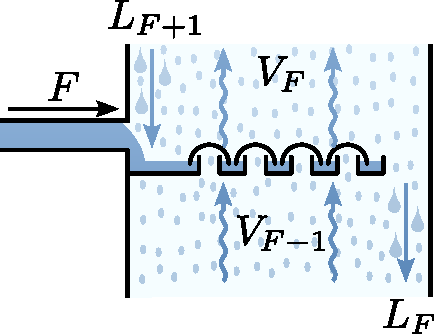
\includegraphics[clip,width=0.5\textwidth]{figures/testfig}
%  \caption{\label{fig:testfig} A test figure.}
%\end{figure}


%
%\section{References}
%You can reference entries in your bib file using the key you have set
%for it like so~\cite{Bannerman_2009}. I can even do cool things like
%say the author of that citation is \citeauthor{Bannerman_2009} and it
%was published in \citeyear{Bannerman_2009}. Or even ask for a full
%citation, like so: \fullcite{Bannerman_2009}.
%
%But you must remember to print the bibliography at the end of every
%chapter!

\printbibliography[heading=thesisChapterBib]
\end{document}
